\documentclass[11pt]{article}
\usepackage{amsmath, amssymb, amscd, amsthm, amsfonts}
\usepackage{graphicx}
\usepackage{tikz}
\usepackage[]{tikz-3dplot}
\usepackage[colorlinks]{hyperref}
\usepackage[nameinlink,noabbrev]{cleveref}
\usepackage{float}
\usepackage{caption}
\usepackage{subcaption}
\usepackage[a4paper, total={6in, 8in}]{geometry}
\usepackage{soul}
\usepackage{enumitem}   

%\oddsidemargin 40pt
%\evensidemargin 40pt
%\marginparwidth 40pt
%\marginparsep 40pt
\topmargin 0pt
\headsep 0pt
\textheight 8.7in
%\textwidth 6in
\linespread{1.2}

\title{Deep Learning FSS22 \\ Assignment 2: CNNs and RNNs}
\author{Timur Michael Carstensen - 1722194}
\date{08.05.2022}


\newcommand{\rr}{\mathbb{R}}

\DeclareMathOperator*{\argmax}{arg\,max}
\DeclareMathOperator*{\argmin}{arg\,min}

\newcommand{\al}{\alpha}
\DeclareMathOperator{\conv}{conv}
\DeclareMathOperator{\aff}{aff}

\begin{document}

\pagenumbering{roman}

\maketitle


\newpage

\tableofcontents

\newpage


\pagenumbering{arabic}

\section{Convolutional Neural Networks}\label{sec:cnn}

\subsection{a)}\label{subsec:cnn-a}
\begin{enumerate}[label=(\roman*)]
\item \textit{3x3 convolutional layer with bias, 1 input channel, 32 output channels, stride 1, padding 1 on each side} 

Input: 28x28x1\\
Output: 28x28x32\\
No. of Parameters: 32 3x3 kernel matrices and 32 bias terms \\

\item \textit{Logistic activation function}

Input: 28x28x32 \\
Output: 28x28x32 \\
No. of Parameters: none\\

\item \textit{2x2 max-pooling layer with stride 2}

Input: 28x28x32\\
Output: 14x14x32\\
No. of Parameters: none \\

\item Linear layer with 10 hidden units

Input: 14x14x32\\
Output: 10 \\
No. of Parameters: 10x6270=62720 \\

\item Log-softmax function

Input: 10 \\
Output: 10 \\
No. of Parameters: none \\
\end{enumerate}

Interpretation: log-probabilities for the 10 different classes of clothing.

\subsection{b)}\label{subsec:cnn-b}
Cf. Code.

\subsection{c)}\label{subsec:cnn-c}
Cf. code.
\subsection{d)}\label{subsec:cnn-d}
Cf. Code.
\subsection{e)}\label{subsec:cnn-e}

\begin{figure}[hbt]
  	\center
  	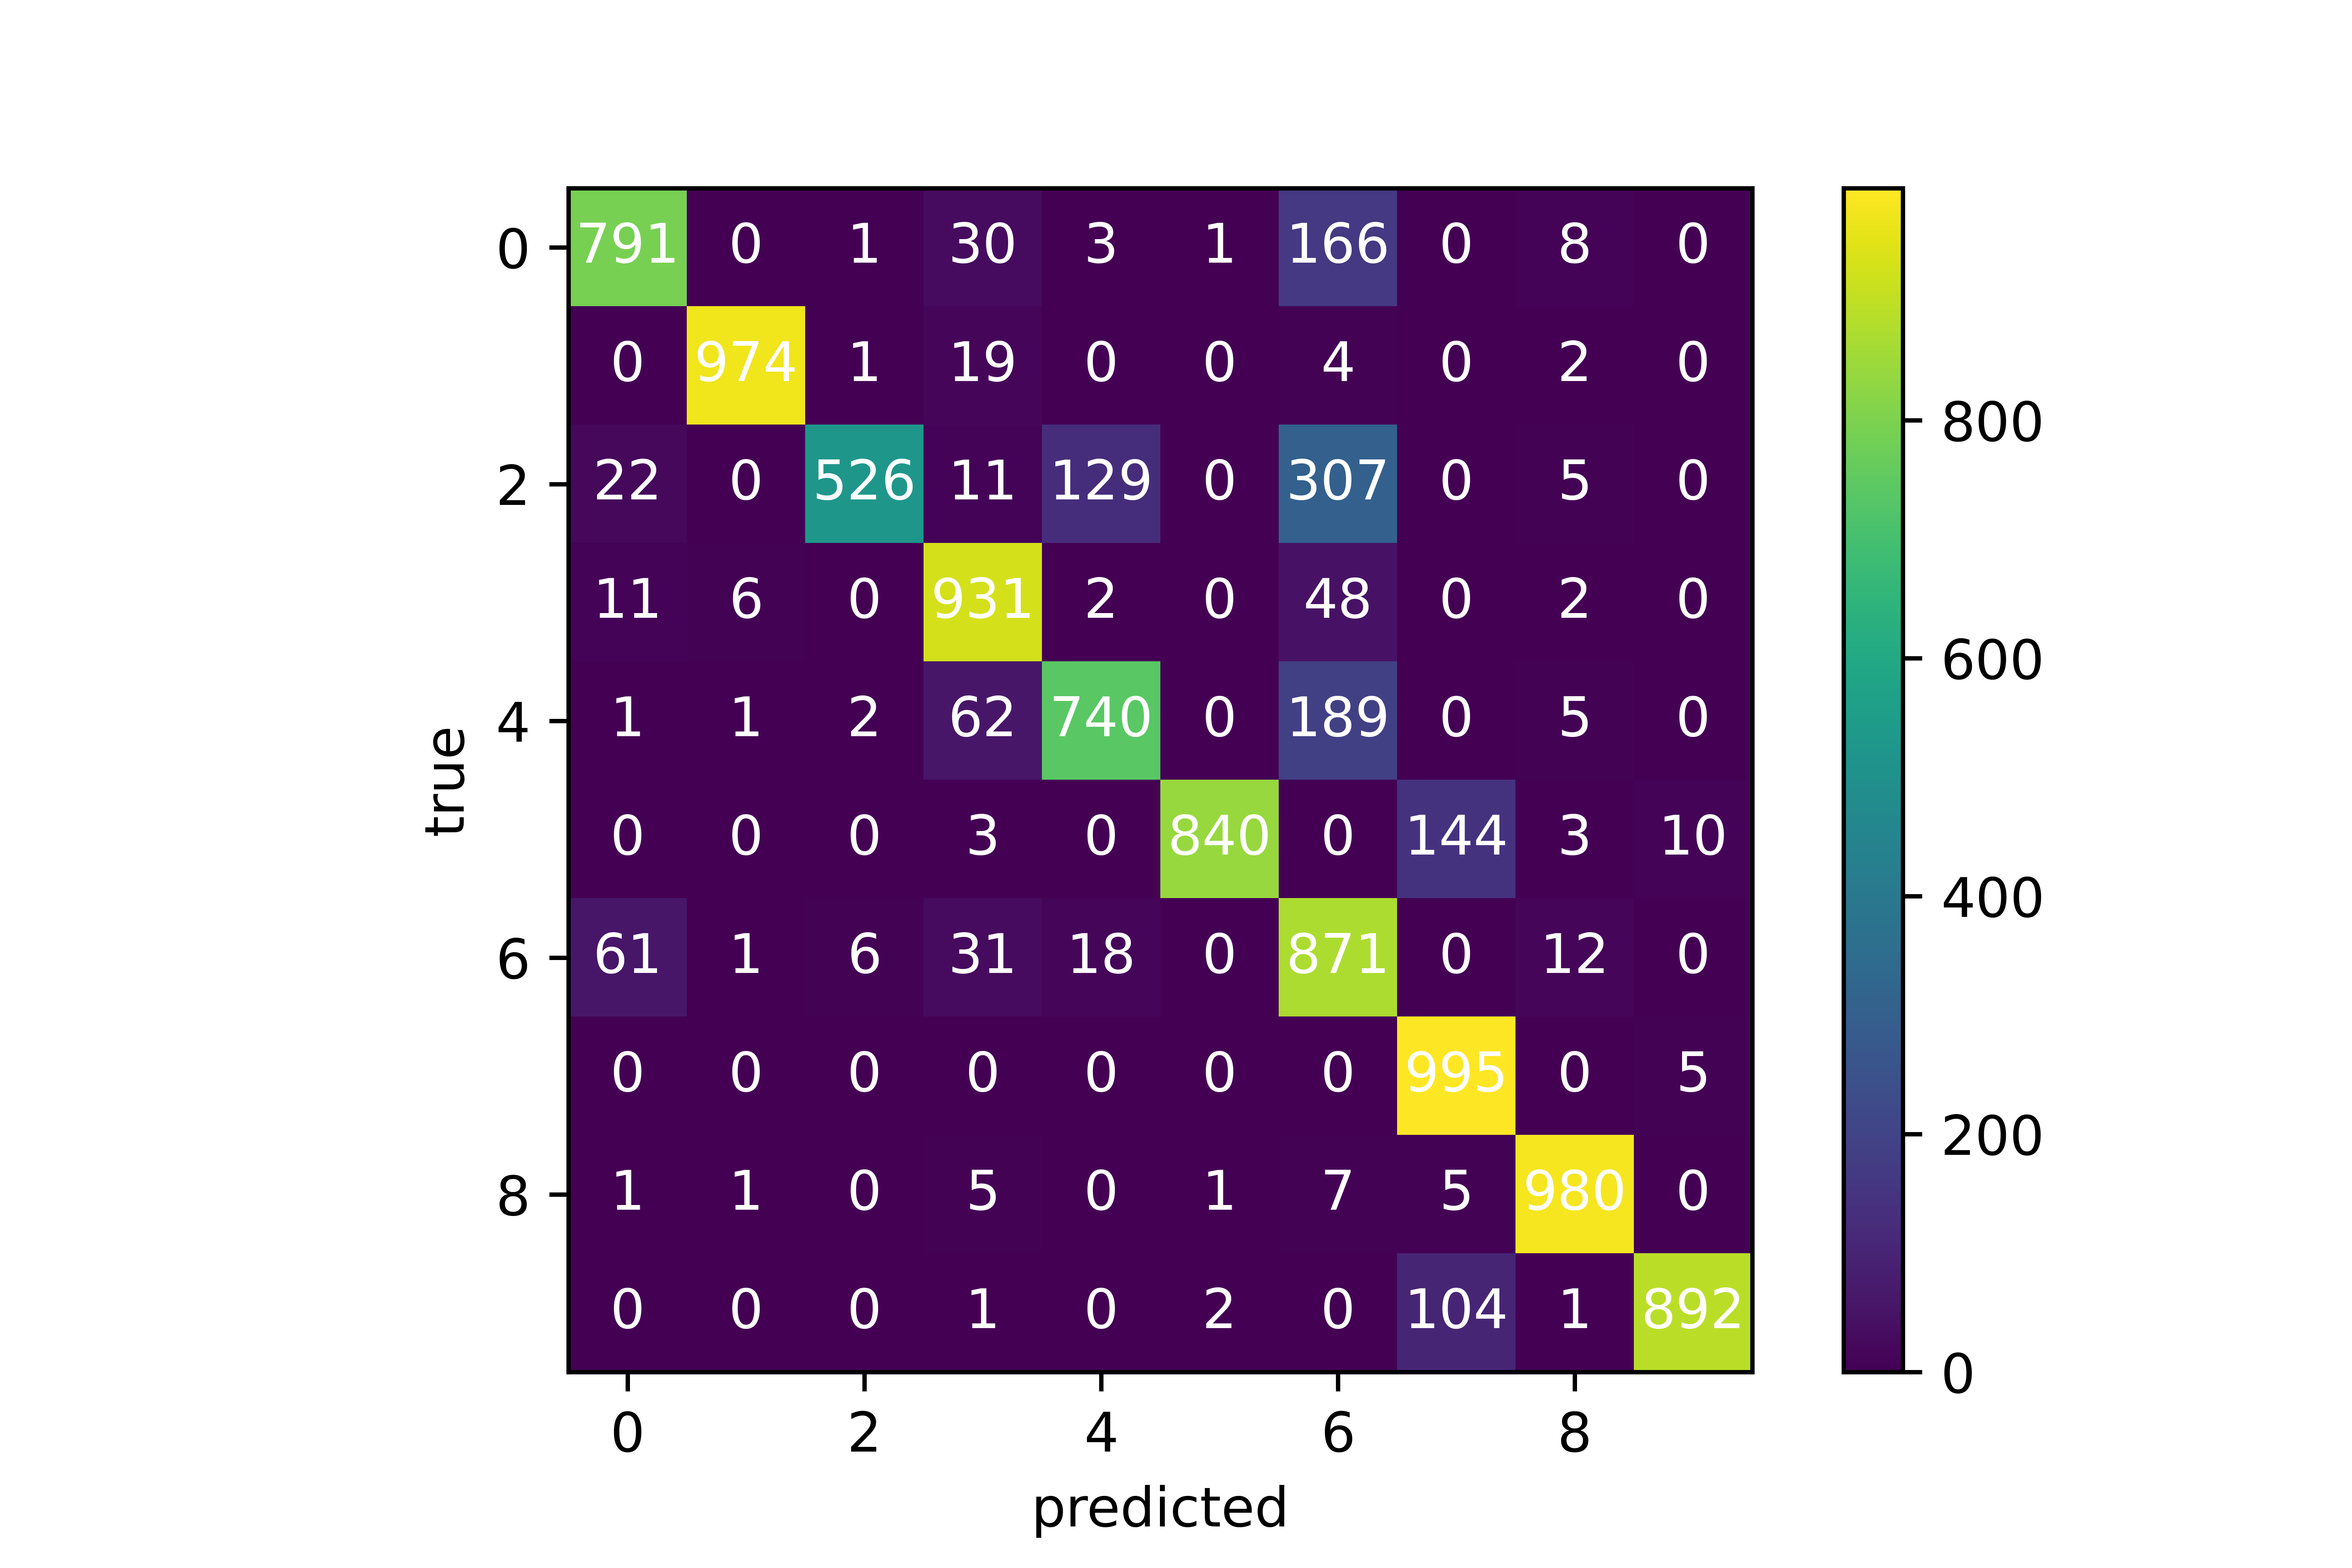
\includegraphics[width=\columnwidth]{assets/conf_mat}
  	\caption{Confusion matrix for the fashion MNIST dataset}
  	\label{fig:f-mnist-conf-mat}
\end{figure}
	


\newpage

\section{Recurrent Neural Networks and Pretraining}\label{sec:rnn}
\subsection{a)}\label{subsec:rnn-a}
Cf. Code.
\subsection{b)}\label{subsec:rnn-b}

\subsection{c)}\label{subsec:rnn-c}

\subsection{d)}\label{subsec:rnn-d}

\subsection{e)}\label{subsec:rnn-e}


\bibliographystyle{alpha}
\bibliography{references}

\end{document}
